\documentclass[a4paper]{article}%
\usepackage[T1]{fontenc}%
\usepackage[utf8]{inputenc}%
\usepackage{lmodern}%
\usepackage{textcomp}%
\usepackage{lastpage}%
\usepackage{geometry}%
\geometry{tmargin=4cm,lmargin=4cm,rmargin=3cm,bmargin=3cm}%
\usepackage{graphicx}%
%
%
%
\begin{document}%
\normalsize%
\section{Jenis Hujan di Indonesia}%
\label{sec:JenisHujandiIndonesia}%
Di area daerah Republik Indonesia dapat kita jumpai tiga macam hujan atau ujan yang turun, yaitu Hujan Frontal, Hujan Orografis, serta Hujan Zenit.%
\subsection{Hujan Frontal}%
\label{subsec:HujanFrontal}%
Hujan frontal adalah hujan yang disebabkan oleh bertemunya angin musim panas yang membawa uap air yang lembab dengan udara dingin bersuhu rendah sehingga menyebabkan pengembunan di udara yang pada akhirnya menurunkan hujan.%


\begin{figure}[h!]%
\centering%
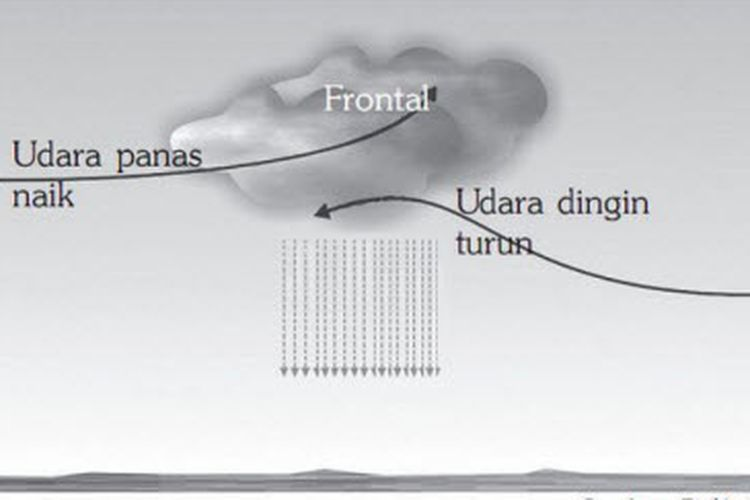
\includegraphics[width=120px]{D:/2. TUTORIAL/Python Excercise/pylatex/contoh-pylatex-5/01-hujan-frontal.jpg}%
\caption{Skema Terjadinya Hujan Frontal}%
\end{figure}

%
\subsection{Hujan Orografis}%
\label{subsec:HujanOrografis}%
Hujan orografis adalah hujan yang diakibatkan oleh adanya uap air yang terbawa atau tertiup angin hingga naik ke atas pegunungan dan membentuk awan. Ketika awan telah mencapai titik jenuh maka akan turun hujan.%


\begin{figure}[h!]%
\centering%
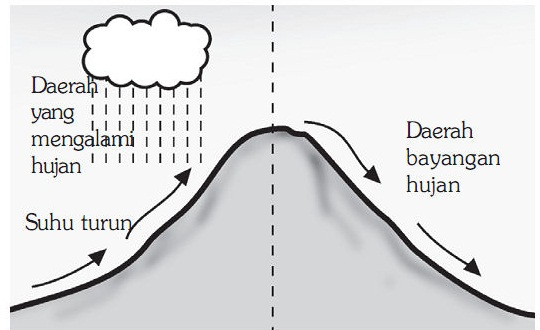
\includegraphics[width=120px]{D:/2. TUTORIAL/Python Excercise/pylatex/contoh-pylatex-5/02-orografis.jpg}%
\caption{Skema Terjadinya Hujan Orografis}%
\end{figure}

%
\end{document}